\chapter{航天器姿态动力学}
\thispagestyle{empty}
\section{动力学建模方法简述}
研究{\color{dy} 角速度$\bm{\omega}_{ba}$的变化与作用力矩之间的关系}的学科称为\dy[姿态动力学]{ZTDLX}。一般有以下几个建模方法。
\vspace*{1em}

\sssection[矢量力学法(牛顿—欧拉法)\index{SLLXF@矢量力学法} \index{NDOLF@牛顿欧拉法}]

采用动力学基本定理(即牛顿运动方程的直接推论),给出系统动力学量与作用于该系统的力之间的关系。即\dy[动量定理]{DLDL}、\dy[动量矩定理]{DLJDL}。
\vspace*{1em}


\sssection[分析力学法\index{FXLXF@分析力学法}]

从系统能量观点出发,运用现代力学的\dy[拉格朗日法]{LGLRF}或\dy[哈密顿法]{HMDF}导出系统的动力学方程。能自动消除物体间的约束力和约束反力,缺点是对于复杂结构,推导工作量大。
\vspace*{1em}


\sssection[矢量力学与分析力学的各种变形方法]

凯恩(Kane)方法、R/W方法、旋量方法、高斯最小约束原理方法等。




\section{刚体的姿态动力学建模原理}
\subsection{单质点的动量矩定理}

如图 \ref{单质点角动量} 所示,坐标系$O'XYZ$是一个惯性坐标系,$O$是其中的一个动参考点,以$O$为原点建立一个动坐标系$oxyz$。

\begin{figure}[!htb]
	\centering
	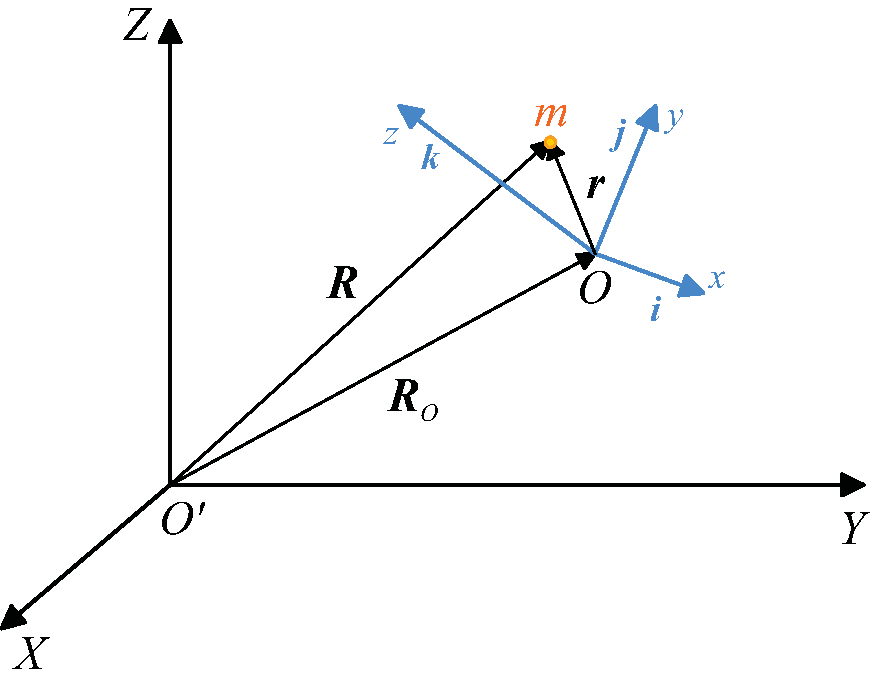
\includegraphics[width=0.4\linewidth]{pic/单质点角动量}
	\vspace*{-1em}
	\caption{质点$m$关于任意参考点$O$的角动量}
	\label{单质点角动量}
\end{figure}

在动坐标系中存在一个质量为$m$的质点,其\dy[线动量]{XDL}为
\begin{equation}
	\bm{p} = m \dot{\bm{R}}
	\nomenclature{$\bm{p}$}{质点的线动量 \nomrefpage}
\end{equation}
其中,$\bm{R}$为质点相对于惯性坐标系的位置向量(绝对位置向量)。

质点$m$的动量$\bm{p}$关于参考点$O$的\dy[角动量]{JDL}(或\dy[动量矩]{DLJ})定义为
\begin{equation}
	\bm{H}^O = \bm{r} \times m \dot{\bm{R}}
	\nomenclature{$\bm{H}^O$}{质点关于参考点$O$的角动量 \nomrefpage}
\end{equation}
其中,$\bm{r}$为质点$m$相对于参考点$O$的位置向量(相对位置向量)。由于$\bm{R} = \bm{R}_O + \bm{r}$,则有$\dot{\bm{R}} = \dot{\bm{R}}_O + \dot{r}$,那么
\begin{equation}
	\ubm{H}^O = \bm{r} \times m \dot{\bm{r}} + \bm{r} \times m \dot{\bm{R}}_O
	\label{H1}
\end{equation}
其中,公式 \eqref{H1} 右侧第一项$\bm{r} \times m \dot{\bm{r}}$称为动坐标系$Oxyz$中的\dy[视角动量]{SJDL},用$\bm{H}^{\underline{O}}$表示;而另一项是因为点$O$运动引起的修正项。
\nomenclature{$\bm{H}^{\underline{O}}$}{质点的视角动量 \nomrefpage}

























